\documentclass[12pt,a4paper,oneside]{book}
\usepackage[utf8]{inputenc}
\usepackage[spanish]{babel}
\usepackage[toc,page]{appendix}
\usepackage{longtable}
\usepackage{amsmath}
\usepackage{amsfonts}
\usepackage{amssymb}
\usepackage{listingsutf8}
\usepackage{color, soul}
\usepackage{paracol}
\usepackage{lipsum}


%%%%%%%%%%%%% Macros para formato 302 %%%%%%%%%%%%%%%%%%%

% Metadata para el PDF a generar 
\usepackage[unicode,
            pdftex]{hyperref}
\hypersetup{
 pdfauthor={Lucas Viera, Bruno Riccardi},
 pdftitle={Sistema de Distribución Multicast mediante SDN},
 pdfsubject={PONER EL SUBTITULO},
 pdfkeywords={PONER PALABRAS CLAVE}
 }

% Numeración y formato de páginas
\usepackage{fancyhdr}
\pagestyle{fancy}
\fancyhf{}
%\fancyhead[lo,le]{\nouppercase{\rightmark}}
\fancyfoot[RO]{\thepage}

\fancypagestyle{plain}{
  \fancyhf{} 
  \fancyfoot[RO]{\thepage}
  \renewcommand{\headrulewidth}{0pt}}
\renewcommand{\headrulewidth}{0pt}


% Indice (estos parámetros se pueden cambiar)
\setcounter{secnumdepth}{3} %para que ponga 1.1.1.1 en subsubsecciones
\setcounter{tocdepth}{3} % para que ponga subsubsecciones en el indice

%% Para incluir imagenes
\usepackage{graphicx}


% Para incluir tablas en español
\renewcommand\tablename{\bfseries Tabla}

% Para incluir listings de código
\renewcommand{\lstlistingname}{\bfseries C\'odigo}

% Para agregar la bibliografía al indice
\usepackage[nottoc,numbib]{tocbibind}


%%%%%%%%%%%%%%%%%%%%%%%%%%%%%%%%%%%%%%%%%%%%%%%%%%%%%%

% Generación del índice
\makeindex

% Empieza el documento
\begin{document}

% Portada (completar con los datos)
\vspace*{\fill}

\begin{center}

\begin{Large}
\textbf{Universidad ORT Uruguay}

\textbf{Facultad de Ingeniería}
\vspace{5cm}
\end{Large}

\begin{huge}
\textbf{Sistema de Distribución Multicast mediante SDN}
\end{huge} 

\begin{Large}
Subtítulo (opcional)
\end{Large}
\bigskip
\bigskip


\textbf{Entregado como requisito para la obtención del título de Ingeniero en Telecomunicaciones.}
\vspace{5cm}

\begin{Large}
\textbf{Lucas Viera - 177863.}\\
\textbf{Bruno Riccardi - 183531.}\\
%\textbf{Nombre Autor 3 - Nro Estud.}\\
\bigskip

\textbf{Tutor: Álvaro Sanchez}
\vspace{2cm}
\end{Large}

\begin{huge}
\textbf{2019}
\end{huge}

\end{center}
\vspace*{\fill}

\thispagestyle{empty}
\newpage




\chapter*{Declaración de autoría}


Nosotros, Bruno Riccardi y Lucas Viera declaramos que el trabajo que se presenta en esta obra es de nuestra
propia mano. Podemos asegurar que:
\begin{itemize}
\item La obra fue produpcida en su totalidad mientras realizábamos el Proyecto.
\item Cuando hemos consultado el trabajo publicado por otros, lo hemos atribuido con claridad.
\item Cuando hemos citado obras de otros, hemos indicado las fuentes. Con excepción de estas citas, la obra es enteramente nuestra.
\item En la obra, hemos acusado recibo de las ayudas recibidas.
\item Cuando la obra se basa en trabajo realizado conjuntamente con otros, hemos explicado claramente qué fue contribuido por otros, y qué fue contribuido por nosotros.
\item Ninguna parte de este trabajo ha sido publicada previamente a su entrega, excepto donde se han realizado las aclaraciones correspondientes.
\end{itemize}

 
\vspace{2cm}


\noindent Incluir las firmas escaneadas en el mismo directorio, con los nombres signature1.jpg, signature2.jpg,.. y descomentar las líneas de abajo.\\

%\includegraphics[scale=0.4]{signature1.jpg} \hfill %\includegraphics[scale=0.4]{signature2.jpg} \hfill %\includegraphics[scale=0.4]{signature3.jpg}\\

XXXX \hfill YYYY \\

01/08/2019 \hfill 01/08/2019



\chapter*{Dedicatoria (opcional)}

No es obligatorio incluirla.



\chapter*{Agradecimientos (opcional)}
No es obligatorio incluirlos. Se trata de un breve reconocimiento a personas o instituciones que de diversas maneras han ayudado en la elaboración del trabajo. 
Asegúrese de usar los nombres correctos y completos de las instituciones y las personas que cite aquí.



\chapter*{Abstract}

Consiste de un resumen del contenido del trabajo, que se usa para difusión y para que el lector potencial sepa en qué consiste el trabajo sin necesidad de leerlo completamente. Puede tener una extensión máxima de 400 palabras. Debe existir coherencia entre el contenido del trabajo final y el abstract. Ver documento 306 (Orientación para títulos, resúmenes o abstracts e informes de corrección de trabajos finales de carrera)



\chapter*{Palabras clave}

Software Defined Networking (SDN), Openflow, Open vSwitch, Multicast, Internet Group Management Protocol (IGMP), Protocol Independent Multicast (PIM), Mininet, Controlador RYU, %Python, Librería, 


\vspace{1cm}

Conjunto de palabras que están directamente relacionadas con el contenido de la obra que además deberán ser incluidas en las
propiedades del archivo PDF para facilitar que el documento sea indexado por los buscadores.


%el siguiente comando genera el índice (no tocar)
\tableofcontents


\chapter{Introducción} 
\label{intro} % para poder referenciarlo después usando \ref{intro}

A modo de ejemplo introducimos el siguiente texto autogenerado:



Ejemplo de lista utilizando itemize:
\begin{itemize}
    \item Primero
    \item Segundo
    \item Tercero\\
\end{itemize}

Ejemplo de enumeración utilizando enumerate:
\begin{enumerate}
    \item Primero
    \item Segundo
    \item Tercero\\
\end{enumerate}

Ejemplo de enumeración anidada utilizando enumerate:
\begin{enumerate}
    \item Primero 
        \begin{enumerate}
        \item Primero
        \item Segundo
        \item Tercero
        \end{enumerate}
    \item Segundo
        \begin{enumerate}
        \item Primero
            \begin{enumerate}
            \item Primero
            \item Segundo
            \end{enumerate}
        \item Segundo
        \end{enumerate}
\end{enumerate}



\section{Ejemplo de Sección}
\label{secc1}

Para incluir una referencia bibliográfica se utilizará el comando cite:~\cite{girard1989}.
Ejemplo de una cita múltiple:~\cite{ranta2012,tcs2015}.\\

También podemos utilizar el comando ref hacer referencia a una capítulo o sección que haya sido indexada con el comando label. Por ejemplo, la introducción, que es el Capítulo~\ref{intro}, o esta misma sección que es la~\ref{secc1}. Ref también sirve para referenciar figuras, como la Figura~\ref{fig1}, que está más adelante en el texto.



\section{Otra sección}

Otra Seccion.




\subsection{Subsección}

Otra subseccion.


\subsubsection{Subsubsección}

Sub sub seccion

\subsection{Subsección}

subseccion

\chapter{Marco Teórico} 
\label{marcoteorico} % para poder referenciarlo después usando \ref{intro}

A modo de ejemplo introducimos el siguiente texto autogenerado:



\section{Software Defined Networking}
\label{marco_sdn}


Software Defined Networking (SDN) se define como la separación física de los planos de Control y Datos, de acuerdo con la Open Networking Foundation (ONF). Esto refiere a la facilitación de la tarea del equipamiento activo de la red (switches, routers, balanceadores etc) dado que la lógica o inteligencia de algoritmos, en un ambiente SDN, se resuelven en un “controlador” programable.

Se trata de la virtualización de funciones relacionadas a la gestión de los elementos activos de una red. Puede entenderse como posibilidad de “programar” o “automatizar” el comportamiento de la red de manera centralizada e independiente del hardware utilizado. 

En la imagen a continuación, se muestra el diagrama presentado por la ONF para mostrar gráficamente la separación de los planos mencionados. En la imagen, se mencionan tres grandes capas: Aplicación, Control e Infraestructura. 

Aca va una imagen si mantenemos lo de la primera entrega

Como se puede observar, la interconexión entre las capas, se da gracias a las “interfaces” que se clasifican en “Southbound Interfaces” y en “Northbound Interfaces” haciendo referencia a la capa de abajo y arriba respectivamente.
	Particularmente, la interfaz “norte” son interfaces de programación (API) - generalmente de alto nivel - que permiten la conexión con elementos externos con diferentes objetivos. Por ejemplo, una API puede ser desarrollada para que la información de la red se muestre en una página web.
	
Finalmente, la interfaz “sur” se trata de la comunicación entre los activos de la red y el controlador. En esta comunicación se hacen especialmente importantes protocolos como Openflow, ya que vinculan comunicaciones provenientes de elementos de la red con el controlador y sin ellos, no se podría generar la separación fundamental de SDN.
	
La filosofía detrás de SDN, similar a la del software Open Source, es decir que busca lograr la desvinculación de hardware y protocolos propietarios junto con la aceptación de estándares abiertos (como Openflow) que permitan la “liberación” o “universalidad” de la programación independientemente de marcas o compañías que lideran los avances con software propietario. 





Para incluir una referencia bibliográfica se utilizará el comando cite:~\cite{girard1989}.
Ejemplo de una cita múltiple:~\cite{ranta2012,tcs2015}.\\

También podemos utilizar el comando ref hacer referencia a una capítulo o sección que haya sido indexada con el comando label. Por ejemplo, la introducción, que es el Capítulo~\ref{intro}, o esta misma sección que es la~\ref{secc1}. Ref también sirve para referenciar figuras, como la Figura~\ref{fig1}, que está más adelante en el texto.



\section{Openflow}
\label{marco_openflow}

Openflow es el protocolo abierto de comunicación utilizado entre el controlador SDN y los switches de la topología. Su especificación está dada por la Open Networking Foundation (ONF) que es el ente, sin fines de lucro, encargado de liderar la transformación de la infraestructura de las redes actuales, de acuerdo a su Misión.

Éste protocolo, es lo que permite la separación de los planos de Control y de Datos descritos en la idea fundamental de SDN. Gracias a él, es posible implementar la inteligencia (Control) en un bloque dedicado a este tipo de procesamiento. Liberando de responsabilidades al equipamiento encargado del switcheo y enrutamiento.

	Los switches que implementan Openflow, contarán con la siguiente estructura lógica en su interior:

aca iria una foto


El funcionamiento de estos switches, vendrá dado por una lógica de “Tablas de flujo” o “Flow Tables”. Cada Tabla de Flujo está compuesta por “entradas de flujo” o “flow entries” que pueden ser agregadas, modificadas o eliminadas según se programe. En cada entrada, se definirán acciones sencillas para ejecutar, por ejemplo, reenvío (o “forwarding”), encapsulamiento o descarte del paquete.

Un paquete puede ser procesado por una tabla de flujo y luego ser enviado a otra tabla del Pipeline para continuar su tratamiento. Esto trae flexibilidad y permite tener gran granularidad a la hora de desarrollar y crear Tablas de Flujo con funciones específicas.

La tablas de flujo en Openflow, tienen una estructura dada compuesta por los siguientes campos:
Match Field: es el criterio de coincidencia que se utilizará para ejecutar la acción. Es el puerto de ingreso del paquete junto con información de la cabecera que está disponible y puede ser manipulada.
Prioridad: para dar un orden de ejecución y es definido por el programador según entienda necesario.
Contadores: para llevar actualizada la cantidad de veces que hubo un “match” con la entrada.
Instrucciones: conjunto de acciones a ejecutar. 
Timeouts: las entradas tienen un tiempo de vida útil acotado por estos timeouts
“Soft timeout”: la entrada se elimina si no hay “match” durante un tiempo mayor al “soft timeout”.
“Hard timeout”: si no es ‘0’, la entrada se elimina luego de existir por un tiempo superior al “hard timeout” sin importar si hubo “match”.
Cookies: puede usarse a modo opcional como valor extra para entradas que dependan de cierta estadística. No se utiliza cuando se procesan paquetes.
	
	Finalmente, se debe aclarar que toda Tabla de Flujo cuenta con una entrada llamada “Table Miss Entry” de prioridad 0, que se utiliza cuando no hubo coincidencia para ninguna de las entradas anteriores. Puede generar que se envíe el paquete al Controlador, que lo descarte o que lo envíe a otra Tabla de Flujo.

	Además de las ya definidas “Flow Entries” el switch Openflow estará compuesto por una Tabla de Grupo o “Group Table” y análogamente, las Tablas de Grupo están formadas por Entradas de Grupo o “Group Entries” que se diferencian en su identificador de grupo o “Group Identifier”.
	
	A su vez, similar a las Tablas de Flujo, las Tablas de Grupo se tienen una estructura dada por los siguientes campos:
Identificador de grupo: es un entero único para diferenciar un grupo de los demás.
Tipo de grupo: se utiliza para representar el comportamiento del grupo. Los switches deben soportar los tipos “indirect” y “all” mientras que opcionalmente pueden soportar a su vez “select” y “fast failover”.
Indirect: grupos que soportan un solo “action bucket”. Permiten varias entradas de flujo y entradas de grupo en un mismo identificador de grupo lo que los convierte en grupos de convergencia rápida y  eficiente. Son los más simples, por lo que es normal que los switches soporten una gran cantidad de ellos en relación a los demás tipos.
All: grupos que ejecutan todos los “buckets” del mismo. Son usados en Multicast y Broadcast dado que permiten clonar efectivamente el paquete en diferentes “buckets”.
Select: grupos que soportan un solo “action bucket”. Los paquetes son procesados por el “bucket” seleccionado de acuerdo a un algoritmo externo a Openflow.
Fast Failover: grupos que ejecutan el primer “action bucket” vivo. Cada “bucket” está asociado a un puerto o grupo que maneja su estado de “vida”. Estos grupos deben implementar un mecanismo para detectar estos cambios de estado.
Contadores: contador que se actualiza cada vez que un paquete es procesado en el grupo.
“Action Buckets”: es el conjunto de acciones a ejecutar sobre un paquete.


\section{Open vSwitch}

Open vSwitch

\section{Multicast}
\label{marco_multicast}

Los métodos de comunicación dentro de una red se pueden clasificar en tres categorías dependiendo en la cantidad de los receptores:
Uno de ellos, es  la comunicación unicast - relación uno a uno - que involucra a un único remitente y receptor. 
Luego se encuentra el método broadcast - relación uno a todos - que consiste en enviar paquetes a todos los integrantes de la red 
Y por último se encuentra el  método Multicast - relación uno a varios - que puede tener variaciones en la cantidad de remitentes, puede ser de uno a muchos o de muchos a muchos.

En la siguiente imagen se muestran las diferencias entre cada método de comunicación.

foto

Una forma de realizar Multicast sería utilizar múltiples conexiones unicast para enviar la misma información a los destinatarios pero no se utiliza de forma eficiente la red y tampoco es escalable debido a que aumenta la carga de trabajo en los emisores y se consume más ancho de banda de la red. Para evitar estos problemas la red realiza copias adicionales a partir de la información original para asegurar que a cada destino le llegue una, generando una menor carga de trabajo y procesamiento en los elementos que conforman la red reduciendo el costo de recursos de esta. Por último provoca que la red sea menos propensa a “embotellamientos”, y por lo tanto que se encuentre más disponible para su uso. 

	Respecto de los envíos de unicast y broadcast, las técnicas de Multicast presentan ventajas para transmitir la misma información a un grupo de receptores generando el uso más eficiente e inteligente del ancho de banda requerido al utilizar sólo una dirección Multicast para el grupo. 



Como en broadcast, Multicast tiene designado un rango de direcciones. Las cuales se encuentran en el rango 224.0.0.0/4, que pueden ser utlizadas para ruteo y en Internet. Presentan como ventaja que la tarjeta de red sólo va a aceptar la información dirigida a una dirección Multicast si la ha solicitado, al contrario de broadcast donde se realiza una inundación en la red.

	Multicast se encuentra basado en el concepto de grupos, formados por los destinatarios que soliciten contenido de determinada dirección Multicast, la cual se puede enviar de forma eficiente en una sola transmisión. Cada integrante de un grupo puede enviar y recibir contenido de la dirección Multicast sin importar su ubicación geográfica, puede estar ubicado en cualquier lugar de Internet o en una red privada.
	
Para unirse o dejar de pertenecer a un grupo Multicast se utiliza el protocolo Internet Group Management Protocol (IGMP). 

IGMP es un protocolo utilizado por sistemas IPV4 para reportar la unión de un host a un grupo Multicast, también para informar la salida de del host del grupo y para obtener el estado de los grupos Multicast formados en la red.

Las funciones de IGMP realizan dos acciones. Cuando un receptor se une a un grupo Multicast, envía un mensaje IGMP para unirse al grupo (Membership Report) con la dirección IP Multicast del grupo al que quiere unirse.
La otra acción está relacionada con la pertenencia dinámica a los grupos. Para esto se designa un switch o un router de la red que sondea de forma periódica mediante un mensaje IGMP de solicitud de pertenencia a grupos (Host Membership Query Message) a los vecinos de la red. De esta forma se determina si se mantienen como miembros activos de grupos. Este mensaje es enviado a la dirección reservada 224.0.0.1, el cual tiene definido un Time to Leave (TTL) de valor uno. Si no se obtiene respuesta al mensaje de pertenencia por parte de un host, se deja de enviarle información y no se anuncia su dirección a las fuentes de datos del grupo al cual pertenecía. 

Hay tres versiones implementadas del protocolo, IGMPv1, IGMPv2 e IGMPv3, las cuales son explicadas en la siguiente sección (IGMP).

Con el protocolo IGMP se obtiene el conocimiento de cómo se encuentran formados los grupos Multicast, en consecuencia se conocen las fuentes de información y los receptores interesados. Resta conocer las rutas que debe utilizar el tráfico Multicast de origen a destino. Esta labor puede ser llevada a cabo por varios protocolos de enrutamiento que se encargan de construir los árboles de tráfico Multicast. Los cuales emplean  uno de los dos métodos básicos dependiendo de la cantidad de miembros que tenga el grupo. En base a ello se encuentran:
Protocolos de Enrutamiento de Modo Denso
Protocolos de Enrutamiento de Modo Disperso

Árboles de distribución Multicast

	Los árboles de distribución son formados a medida que los receptores se van uniendo o saliendo de los grupos Multicast. Son determinados por los caminos de enrutamiento del tráfico desde el origen a los receptores. 
	Hay dos tipos de árboles:
Short Path Tree (SPT)
Rendezvous Point Tree

	Short Path Tree
	Los SPT también llamados Árboles Basados en Origen definen un árbol de distribución para cada origen de tráfico Multicast que lo conecta con los receptores. Este tipo de árboles son usados por protocolos de Multicast en modo denso como DVMRP, PIM-DM y MOSPF. Para enviar el tráfico emplean el camino más corto entre el origen y destino tomando en cuenta la métrica de acuerdo a los saltos o la métrica de velocidad, referida al camino de menor retraso. La siguiente figura muestra tres árboles SPT desde la fuente hasta tres receptores. Gracias a esto crea una ruta óptima entre el origen y los participantes, garantizando un tiempo mínimo de retardo.

foto

Rendezvous Point Tree	
	En los RPT el camino del tráfico se encuentra arraigado al router designado como Rendezvouz Point (RP) y no a la fuente del tráfico. Este tipo de árboles son usados por el protocolo PIM-SM. Los routers de la red encaminan la información de varias fuentes al RP y el RP se encarga de redirigirla a los receptores. En el modelo RPT los routers no tienen que conocer donde se ubican las fuentes de cada grupo Multicast, sólo necesitan conocer dónde se encuentra el RP. El RP debe descubrir las fuentes de cada grupo Multicast. En la siguiente imagen se muestra un ejemplo de árbol RPT.

foto

Multicast Forwarding 

En una transmisión unicast el tráfico es enviado a través de la red por un solo camino, de origen a destino. En Multicast la fuente envía información a una dirección que representa un grupo Multicast, el router debe identificar qué dirección está en sentido ascendente (hacia la fuente) y cuál se encuentra en sentido descendente. El concepto de encaminar tráfico lejos de la fuente, o sea hacia al receptor, se denomina Reverse Path Forwarding (RPF) .

	RPF permite a los routers encaminar tráfico Multicast hacia abajo por el árbol de distribución. Utiliza la tabla de ruteo unicast para determinar sus vecinos descendentes y ascendentes, de esta forma sólo va a encaminar un paquete si es recibido por la interfaz ascendente. Si el paquete es recibido por la interfaz descendente, termina siendo descartado. Gracias a este método de transmisión se evitan los loops en las redes que implementan Multicast.






\subsection{Multicast en Capa 2}



\subsection{Multicast en Capa 3: IP Multicast}

ip multicast


\section{Internet Group Management Protocol (IGMP)}

\subsection{IGMPv1}

Es la primera versión de IGMP y consta de sólo dos tipos de mensajes de control, Membership Report (MR), emitido por los hosts, y Membership Query (MQ), emitido por el router. No implementa un mecanismo para que un host abandone un grupo Multicast. Los receptores envían un MR y el router designado lo registra en el grupo. El router envía periódicamente un MQ para comprobar si al menos un receptor continúa interesado en recibir tráfico del grupo. 

\subsection{IGMPv2}

IGMPv2 implementa la misma funcionalidad básica de IGMPv1. Se diferencia en que introduce un nuevo tipo de mensaje para abandonar el grupo Multicast, llamado Leave Group (LG). Gracias a este mensaje se identifica inmediatamente los receptores que ya no desean pertenecer al grupo Multicast. Cuando un host quiere abandonar el grupo envía un mensaje LG a la dirección Multicast 224.0.0.2. El router envía un mensaje MQ al grupo que el host quiere abandonar, si el host no responde con un MR, entonces se le deja de enviar tráfico al host. Si no se recibe ningún MR de parte del grupo se elimina el grupo Multicast.

IGMPv2 especifica dos modalidades de consulta, General Query y Group Specific Query. General Query es la utilizada por IGMPv1 y Group Specific Query permite realizar la consulta a los integrantes de determinado grupo.


\subsection{IGMPv3}

IGMPv3 agrega con respecto a las versiones anteriores, la funcionalidad de permitir que un receptor solicite recibir o dejar de recibir tráfico de una fuente o varias determinadas pertenecientes a un grupo. También añade otro tipo de mensaje de consulta, Group and Source Specific Query, para preguntar qué receptor continúa interesado en recibir tráfico Multicast de varias fuentes o una fuente concreta.

\subsection{Protocolos de enrutamiento}

 Protocolos de enrutamiento

Los protocolos de enrutamiento de Multicast IP siguen uno de los dos enfoques básicos determinados por la distribución de los miembros del grupo Multicast en toda la red.

El primer enfoque se basa en suponer que los miembros del grupo Multicast se distribuyen densamente en la red, es decir, muchas de las subredes contienen al menos un receptor del grupo. Esto se denomina Enrutamiento de Modo Denso y se basa en una técnica llamada inundación (se le envía el tráfico a todos los integrantes de la red) para propagar la información de todas las fuentes de tráfico Multicast de la red.
	
El segundo enfoque se basa en que los miembros del grupo se encuentran muy dispersos en la red y el ancho de banda disponible no es abundante. Esto ocurre en muchas regiones de Internet. En este caso inundar la red causaría un uso innecesario del ancho de banda disponible provocando el saturamiento de la red. Por lo tanto este modo debe emplear técnicas más selectivas para configurar los árboles de Multicast y se le llama Enrutamiento de Modo Disperso.


Protocolos de Enrutamiento de Modo Denso
	
Entre los protocolos de enrutamiento de este modo existen los siguientes:
Distance Vector Multicast Protocol (DVMRP)
Multicast Open Shortest Path First (MOSPF)
Protocol Independent Multicast Dense Mode (PIM-DM)


Protocolos de Enrutamiento de Modo Disperso
	
Los protocolos de Enrutamiento de Modo Disperso es utilizado para grupos de receptores dispersos y alejados, no realizan una inundación como los de modo denso sino que envían tráfico sólo a los receptores interesados. Debido a esto son implementados en entornos donde se tiene disponible un ancho de banda acotado. Un protocolo de enrutamiento de este modo es el siguiente:
Protocol Independent Sparse Mode (PIM-SM)


\section{Protocol Independent Multicast (PIM)}

PIM es un protocolo desarrollado con el objetivo de estandarizar el enrutamiento Multicast que puede proporcionar un enrutamiento entre dominios a través de Internet, independientemente de los mecanismos proporcionados por los protocolos de enrutamiento unicast. Presenta dos modos operativos, uno para grupos Multicast densamente distribuidos (PIM-DM) y otro para grupos de distribución dispersa (PIM-SM).


\subsection{PIM Sparse Mode}

En PIM-SM no se envía tráfico Multicast salvo que un receptor lo requiera. Para distribuir el tráfico se utilizan árboles RPT donde el RP se fija como punto de encuentro para los paquetes que se envían de las fuentes a los hosts. Entonces cada router si recibe tráfico Multicast lo va a enviar al RP y cada router que quiera recibir tráfico se va a dirigir al router RP.

	A continuación se explica el funcionamiento del protocolo mediante un ejemplo. El ejemplo consiste en un servidor, que se encuentra realizando streaming a la dirección de Multicast 239.1.1.1 y el router R6 recibe un IGMP Membership Report desde un host conectado que desea recibir tráfico desde el servidor.

foto

El router R6 va a poder encontrar el servidor gracias al router RP, como fue mencionado anteriormente. El router R6 puede encontrar el RP de dos formas. Una es configurando manualmente la dirección del RP en cada router de la red, la otra es gracias a un protocolo que realiza la función de descubrir la red.  
	
Para recibir el tráfico Multicast el host debe enviar un mensaje IGMP Membership Report el router R6. Luego el router envía el mensaje hacia el RP para notificar del host interesado en el tráfico. En la siguiente imagen se muestra lo mencionado anteriormente.

foto

Cuando el RP recibe el mensaje IGMP comienza a enviar el tráfico hacia el host. El concepto de unirse al RP se le llama Rendezvous Path Tree (RPT). Cada grupo Multicast puede tener diferentes RP designados y también varias fuentes de tráfico. En la siguiente imagen se muestra el RPT formado.

foto

Por último PIM-SM tiene la funcionalidad de calcular la ruta más corta desde la fuente del tráfico al receptor. Cambia de un Rendezvous Path Tree a un Short Path Tree. Cuando obtiene la ruta más corta envía mensajes de tipo prune para eliminar la ruta utilizada anteriormente. De esta forma no se va a utilizar más el RP para el tráfico hacia ese receptor desde esa fuente.

En la siguiente imagen se muestra el cambio realizado en la ruta.


\subsection{PIM Dense Mode}

PIM-DM.
	PIM-DM es un protocolo de enrutamiento de modo denso, que construye árboles de tipo SPT inundando de tráfico Multicast la red y luego utiliza  pruning para eliminar las ramas donde no se encuentren receptores. 
	En la siguiente imagen se muestra la inundación generada en la red.

foto

Cada router que reciba el tráfico Multicast va realizar una inundación en la red, provocando problemas. Uno son los loops de ruteo Multicast. Para evitarlos, los routers que no solicitaron el tráfico Multicast envían mensajes de tipo prune a los upstream routers (routers de donde se recibe el tráfico Multicast). Los mensajes prune se envían cuando el router no tiene hosts conectados directamente interesados en el tráfico Multicast, cuando no hay downstreams (routers a los cuales se envía el tráfico Multicast) routers interesados en el tráfico Multicast y cuando se recibe tráfico en una interfaz que no funciona como RPF.
	Luego de eliminar los caminos no deseados para el tráfico se termina obteniendo lo que se llama un Short Path Tree (SPT). En la siguiente imagen se representa como queda el recorrido del tráfico.


foto

\subsection{Modelos de comuicación}

Multicast se clasifica en dos formas según el modo en que se envía la información. Uno es el Any Source Multicast (ASM) y el otro Source Specific Multicast (SSM). 
	
En Any Source Multicast se pueden tener varios servidores que envían información en un mismo grupo, utilizando la forma de intercambio de datos muchos a muchos. Para soportar el modelo muchos a muchos la red debe ser responsable del descubrimiento de la fuente. Cuando un host requiera unirse a un grupo, la red tiene que determinar todas las fuentes del grupo y enviárselas al host.
	
Source Specific Multicast se utiliza el método de envío de uno a muchos y la red no es responsable de saber dónde se encuentra la fuente de datos, ahora los hosts son los encargados de realizar esa función. Los hosts cuando se unen a un grupo especifican la fuente de donde quieren recibir la información y el grupo Multicast.
	
ASM y SSM no son protocolos, son modelos de servicio. Diferentes protocolos son implementados para poder realizarlos. Por ejemplo para SSM se utilizan los protocolos PIM-SM e IGMPv3.


\section{Open vSwitch}

Open vSwitch

\section{Mininet}

El software Mininet, es un emulador gratuito de elementos de redes SDN que puede representar virtualmente switches, routers y hosts clientes que emulan el kernel de Linux. Funciona  ya sea en un sistema Linux así como máquina virtual con otro sistema operativo lo que lo hace muy flexible para ambientes de investigación, desarrollo y enseñanza.

Además, permite la rápida creación de topologías complejas, testeo de desarrollos particulares, simulación de redes y todo sobre una misma consola. Es un proyecto de la ONF y por lo tanto, soporta el protocolo Openflow. En la imagen a continuación, se representa la “virtualización” posible gracias a Mininet, de los elementos físico de una posible red que se quiera emular:

Aca iria una foto.

Mininet provee ventajas respecto a los recursos necesarios para correr, la velocidad de booteo y la versatilidad respecto a los sistemas sobre los que corre. Además, es gratuito y de código abierto y con una comunidad que ha generado material y cursos útiles en varios sitios de internet.

Entre las ventajas, se contempla que la emulación de hosts, se hacen sobre el mismo kernel y esto permite la utilización de herramientas de networking y de línea de comandos disponibles en Linux. Por ejemplo, se pueden correr Scripts desde línea de comandos, se pueden correr servicios HTTP de pruebas, capturar paquetes con “tcpdump”, utilizar la herramienta “iperf” para testear capacidades y generar conexiones simultáneas o “scapy” para la generación de paquetes customizados entre muchas otras herramientas.

Respecto a las desventajas de Mininet, se encuentra la limitante física que impone el CPU y el ancho de banda disponible en el servidor donde corra. No es un emulador utilizado en ambientes de producción, sino más bien en entornos de investigación y desarrollo a pequeña o mediana escala.

foto



\section{Controlador RYU}

El presente Proyecto será desarrollado utilizando aplicaciones del controlador RYU. Su significado, del japonés, es “flujo”. Este controlador, provee componentes de software sobre los cuales se pueden construir aplicaciones complejas para implementaciones de SDN. 

Es un software abierto cuyo código está disponible para todo público y soporta protocolos como Openflow, Netconf, OF-Config, etc. Está implementado totalmente en Python. Se integra con una gran variedad de switches reales de diferentes marcas y es compatible con Openstack.

Como desventaja, se podría señalar la falta de una interfaz gráfica para su configuración, como tienen otros controladores de SDN, aunque sí tiene un entorno gráfico para la visualización de las topologías llamado “Ryu Topology Viewer”.

Finalmente, dentro de las funcionalidades implementadas que vienen embebidas con RYU, se pueden mencionar el controlador “simple_switch.py” que está implementado para varias versiones de Openflow y, básicamente, permite el conocimiento de los host conectados a cierto switch y el armado de una tabla de direcciones MAC.


\chapter{Otro Capítulo}

Notar quue se genera una página nueva al iniciar un capítulo.

pepitp
\section{Otra Sección}

En esta sección incluimos una figura.
\begin{figure}[ht]
 \centering
 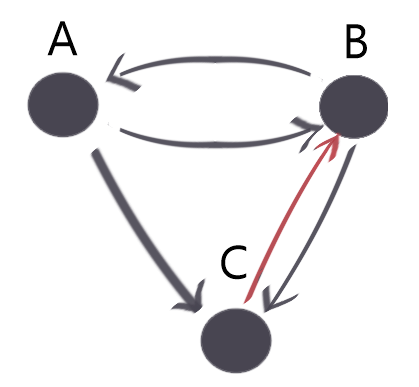
\includegraphics[width=0.5\textwidth]{grafo.png}
 \caption{Figura de ejemplo.}
 \label{fig1}
\end{figure}

\subsection{Otra Subsección}
\lipsum[2-5]

\chapter{Conclusiones}
\lipsum[1-6]




\bibliographystyle{IEEEtran}
%%bibliography
%% No borrar estas dos líneas. Revisar de tener los archivos IEEETran y biblio.bib en la misma carpeta
%% si no están y no anda, correr el compilador de latex varias veces. Primero el bibtex, luego pdflatex, luego pdflatex otra vez.
\bibliography{biblio}


\appendix %A partir de acá los capítulos se enumerarán A, B, C, etc


\chapter{Nombre del Apéndice 1} 
\lipsum[1]
\section{Una Sección}
\lipsum[2-3]
\subsection{Una Subsección}
\lipsum[4-6]

\chapter{Nombre del Apéndice 2} 
\lipsum[6-9]

%\end{appendices}





\end{document}

